\documentclass{beamer}

\usepackage[utf8]{inputenc}
\usepackage{graphicx}
\graphicspath{{img}}

\title{Moogle!}
\author{Ramón Hernández Camacho}
\date{Julio 2023}
\usetheme{CambridgeUS}

\begin{document}

\maketitle

\begin{frame}{Breve Descripción}
    Moogle! es una aplicación Web creada con el objetivo de buscar un texto determinado
    en un conjunto de documentos de acuerdo a la relevancia que tiene el conjunto de
    palabras introducidas por el usuario (Query) en cada documento.
    \begin{center}

        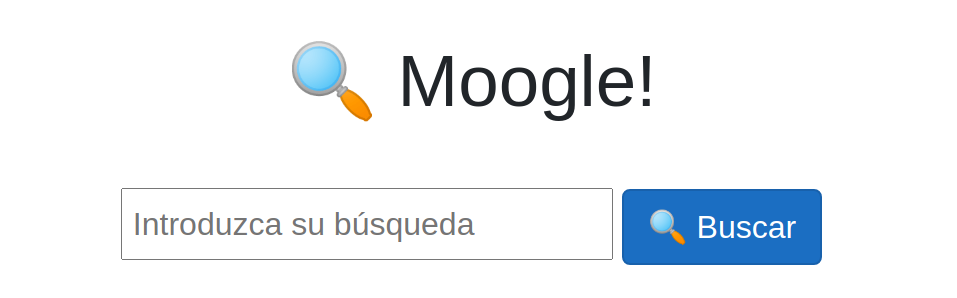
\includegraphics[width=12cm]{moogle.png}

    \end{center}


\end{frame}

\begin{frame}{Funcionamiento General}
    A través del uso del TF-IDF (Frecuencia
    de Término- Frecuencia Inversa de Documento) y la fórmula del coseno es capaz de determinar cuan similares son 2 documentos entre sí.
    \begin{figure}[h]
        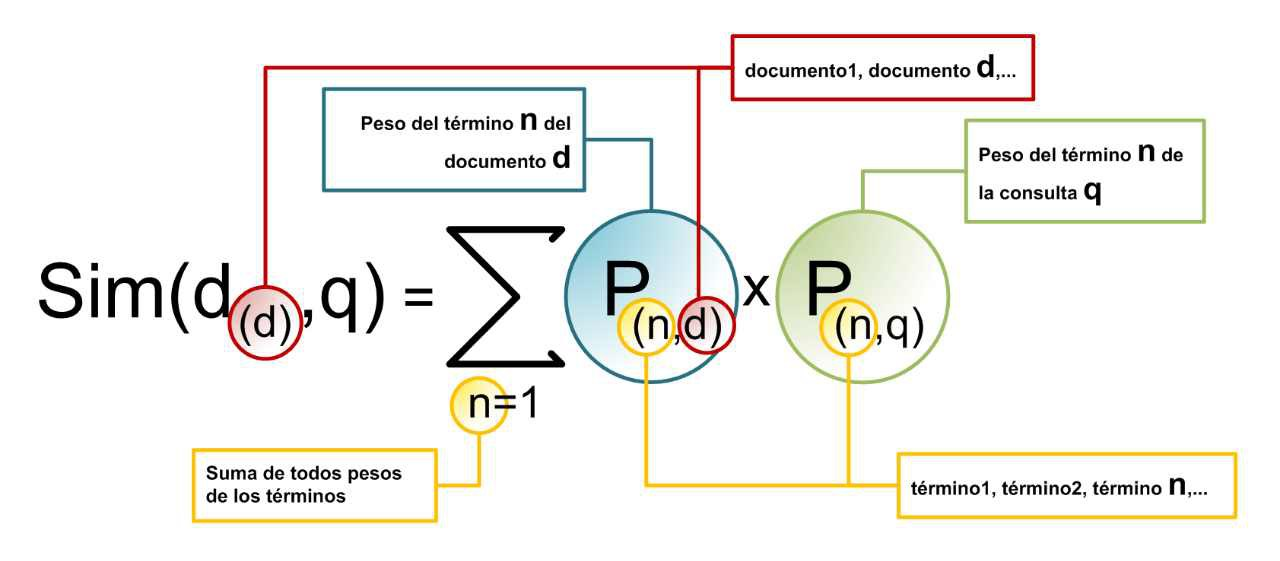
\includegraphics[width=10cm]{1.jpg}
        \caption{Formula que representa como calcular la similitud entre 1 documento y la
            query solo teniendo en cuenta el TF-IDF.}
    \end{figure}
\end{frame}
\begin{frame}{Funcionalidades Adicionales}

    \begin{itemize}
        \item Operador * : Permite aumentar la relevancia de una palabra.
        \item Operadores ! y \^\ : Eliminan de los resultados los documentos que contienen y no contienen cierta palabra.
        \item Operador \~\ : Aumenta la relevancia de un documento mientras mayor sea la cercania de las 2 palabras entre las que se coloque el operador.
        \item Recomendacione : Si la cantidad de resultados es muy pequeña se le sugerirá al usuario una búsqueda que arroje mayor cantidad de resultados.
        \item Otros : Al presionar "Enter" se realiza la busqueda escrita en la barra , al presionar sobre la sugerencia esta realiza la búsqueda sin necesidad de escribirla.
    \end{itemize}
\end{frame}

\end{document}